\documentclass{article}
\graphicspath{{/home/david/Book/Chapters/2.Vectors/Vectors/pic/}}

% !TeX root = ../../../Mainfile/book.tex



\begin{document}


\subsection{Vector properties}

\begin{align*}
\vec{v}  = \color{rooj} \begin{bmatrix} 4 & 3 \end{bmatrix}  \color{black}
 =  \color{groen} \begin{bmatrix} 4 \\ 3 \end{bmatrix}  \color{black}
\end{align*}

Here we have an example of  a (\textbf{2-dimensional}) vector, written both as a \color{rooj} row vector \color{black} and a \color{groen} column vector\color{black}.
All that a vector is is a \textbf{length} and a \textbf{direction}


The length of a vector is written as $|\vec{v}|$ and found with the Pythagorean-theorem:

\[
|\vec{v}| = \sqrt{4^2 + 3^2} = \sqrt{25} = 5
\]

and its direction is written $\theta_{\vec{v}}$ and calculated using absolute classic geometry

\[
\theta_{\vec{v}} = \tan^{-1}\frac{3}{4} 
\]

\begin{minipage}{0.45\textwidth}
\begin{figure}[H]
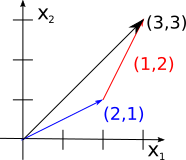
\includegraphics[width = 0.9\linewidth]{1.png}
\end{figure}
\end{minipage} \hfill
\begin{minipage}{0.55\textwidth}
\begin{flushleft}
We can easily draw 2-dimensional vectors on an xy-plane. Here the vector $\vec{v}$ appears twice, one starting from $(0,0)$ and the other from $(2,-4)$.
\end{flushleft}
\end{minipage}



\end{document}